% --------------------------------------------------------------
% This is all preamble stuff that you don't have to worry about.
% Head down to where it says "Start here"
% --------------------------------------------------------------
 
\documentclass[12pt,a4paper,twoside]{article}
\usepackage[margin=1in]{geometry} 
\usepackage{amsmath,amsthm,amssymb,listings,graphicx}
\usepackage[usenames,dvipsnames]{xcolor}
\usepackage{fancyhdr}
 
\pagestyle{fancy}
\fancyhf{}

 
\newcommand{\N}{\mathbb{N}}
\newcommand{\Z}{\mathbb{Z}}
\newcommand{\set}[1]{\ensuremath{\left\{{#1}\right\}}}
\newcommand{\bracket}[1]{\ensuremath{\left [{#1}\right]}}
\newcommand{\brocket}[1]{\ensuremath{\left\langle{#1}\right\rangle}}
\newcommand{\norm}[1]{\left\|{#1}\right\|}
\newcommand{\ceil}[1]{\ensuremath{\left\lceil {#1}\right\rceil}}
\newcommand{\floor}[1]{\ensuremath{\left\lfloor {#1}\right\rfloor}}
\newcommand{\paren}[1]{\ensuremath{\left({#1}\right)}}
 
\newenvironment{exercise}[2][Exercise]{\begin{trivlist}
\item[\hskip \labelsep {\bfseries #1}\hskip \labelsep {\bfseries #2.}]}{\end{trivlist}}
\newcommand{\solution}{\medskip\noindent{\textit{Solution:}}\quad}

\definecolor{dkgreen}{rgb}{0,0.6,0}
\definecolor{gray}{rgb}{0.5,0.5,0.5}
\definecolor{mauve}{rgb}{0.58,0,0.82}

\lstset{frame=tb,
  language=R,
  aboveskip=3mm,
  belowskip=3mm,
  showstringspaces=false,
  columns=flexible,
  basicstyle={\small\ttfamily},
  numbers=none,
  numberstyle=\tiny\color{gray},
  keywordstyle=\color{blue},
  commentstyle=\color{dkgreen},
  stringstyle=\color{mauve},
  breaklines=true,
  breakatwhitespace=true,
  tabsize=3
} 

\lhead{\color{Maroon}David Plotz working with Taha}
\rhead{\color{Maroon}Stat. 6509}
\chead{\color{Maroon}Final Project}
\cfoot{\thepage}

\begin{document}

% --------------------------------------------------------------
%                         Start here
% --------------------------------------------------------------
In this report we will create a regression model to predict the wages of a worker in the United States given several predictor variables. Besides for the predictor variables given to us, we will also like to include the interaction between several of these predictor variables to see if any of these interactions are also useful for prediction, including the interaction of education with itself (i.e., the square of eduction), the interaction of education with experience, and the interaction between how long someone has been at a company and whether they live in a metropolitan area. We were particularly interested in the difference between the wages of females versus males and we therefore included every linear multiplicative interaction that was possible between the female indicator and all other predictor variables. We then selected several models that seemed to give a good fit to the log wages. Finally we used these models and cross-validated them to select the best model. Using this model, we were able to predict the wages of an individual to an accuracy of plus or minus 3 dollars 90 percent of the time. \\     
	
Before starting to make our model, we first checked for outliers in our data set. One of the data points was particularly troubling as the person was making less than the minimum wage. We decided at the outset to drop this data point from our data set because we figured it was probably an error in the data collection methods.\\
	
After deleting this outlyer, we examined the histogram of wages. As you can see, below to the left, the wages are skewed to the right, we therefore used the log of wages instead, which I have plotted on the left.
\begin{center}
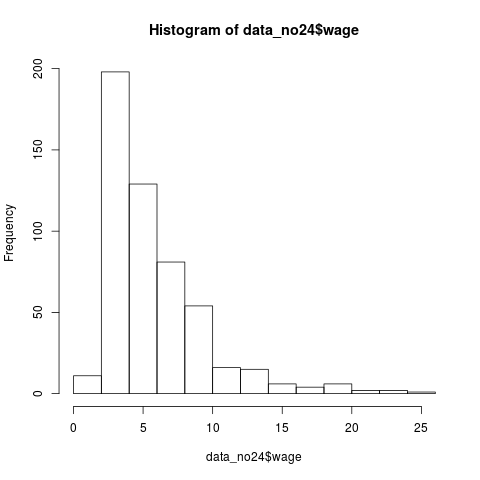
\includegraphics[scale=.2]{plot2.png}
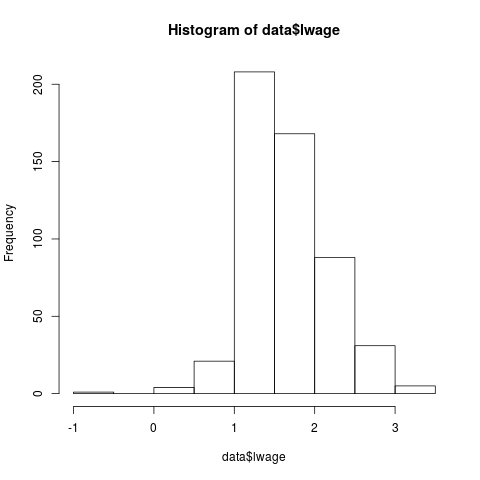
\includegraphics[scale=.2]{plot1.png}
\end{center}

Before looking at the interactions that were possible, we wanted to make sure that a linear interaction was appropriate for each of the numeric explanatory variables. What we found was that experience, education and tenure all showed curvature. A lack-of-fit test confirmed our suspicions. We therefore included education squared, experience squared, and the log transformation of tenure into our model.\\

A preliminary study of the data shows us that we should use polynomial relationship between the lwage, our dependent variable and experience and education, two of our independent variables.\\
The transformation of tenure to the log version was tested with a lack of fit test between lwage and tenure in SAS, and lack of fit was significant in the simple version while it was insignificant in log version. So I decided to use log tenure instead of tenure and tenure squared.\\
\begin{tabular}{l l}
%\includegraphics[scale=.4]{Rplot01}&

%\includegraphics[scale=.4]{Rplot03} \\ 

%\includegraphics[scale=.4]{Rplot04}&

%\includegraphics[scale=.4]{Rplot05}\\
\end{tabular}

Although from the scatterplot matrix there seems to be strong correlation between tenure and experience, a possible collinearity problem, the correlation matrix shows us that the correlation between these two is not bigger than .9 which is our cutoff point, hence, they can both be included in the model.\\
%\includegraphics[scale=.9]{Rplot02}


Our data shows that women are discriminated against in their wages, but checking at the interactions, only women who are married and/or long tenure, are the targets, non of the other variables tend to have a significant interaction with gender, while adding these two would explain most of the variance in wages of the women, hence, after these two are added, the gender variable itself would become insignificant in the model
	*p-value of the hypothesis test if the gender variable should be in the model afterward become .6.  
\begin{tabular}{c c}
%\includegraphics[scale=.3]{MSGN} &
%\includegraphics[scale=.4]{LTGN}\\
%\includegraphics[scale=.35]{gnbf} &
%\includegraphics[scale=.35]{gnaf}\\
\end{tabular}




\end{document}
